\documentclass[12pt]{article} % Увеличенный базовый шрифт
\usepackage[utf8]{inputenc}
\usepackage[T2A]{fontenc}
\usepackage[english,russian]{babel}
\usepackage{amsmath}
\usepackage[left=1.5cm, right=1.5cm, top=1.5cm, bottom=1.5cm]{geometry}



\usepackage{longtable}
\usepackage{graphicx}
\usepackage{array}

\usepackage{wrapfig}
\usepackage{siunitx} % Required for alignment
\usepackage{subfigure}
\usepackage{multirow}
\usepackage{rotating}
\usepackage{caption}
\graphicspath{{pictures/}}

\usepackage{indentfirst}
\setlength{\parindent}{1cm}

\title{\begin{center}Вопрос по выбору:\end{center}
Уравнения моделей неидеальных газов}
\author{Струков Олег Игоревич \\ Б04-404}
\date{}

\begin{document}

    \pagenumbering{gobble}
    \maketitle
    \newpage
    \pagenumbering{arabic}

\section*{Введение}

Кроме модели Ван-дер-Ваальса было предложено множество иных эмпирических или полуэмпирических уравнений состояния реальных газов, которые в различных условиях лучше соответствуют экспериментальным данным. Наиболее известными из них являются

Уравнение Дитеричи:
\begin{equation}
P(V - b) = RT \exp\left(-\frac{a}{RTV}\right),
\end{equation}

Уравнение Бертло:
\begin{equation}
\left(P + \frac{a}{TV^2}\right)(V - b) = RT,
\end{equation}

Уравнение Клаузиуса:
\begin{equation}
\left(P + \frac{a}{T(V + c)^2}\right)(V - b) = RT,
\end{equation}

Уравнение Камерлинга — Оннеса:
\begin{equation}
PV = RT\left(1 + \frac{B_2}{V} + \frac{B_3}{V^2} + \ldots\right).
\end{equation}

В данном вопросе по выбору я иследую, из каких предположений выводятся данные уравнения и сравню условия их применимости.

\section*{Уравнение Дитеричи}
\subsection*{Учёт размеров молекул}

В первую очередь, аналогично модели Ван-дер-Ваальса, считая молекулы шарами радиуса r, стоит учесть, что центры двух из них не могут сблизиться на расстояние меньше 2r. 
Таким образом, ограничение объёма на одну молекулу в газе составляет $\dfrac{1}{2}\left(8\cdot\dfrac{4}{3}\pi r^3\right) = 4V_0 $, где $V_0$ -- объём одной молекулы.
Беря за основу уравнение Менделеева-Клапейрона для одного моля газа, получаем улучшенную модель: $P(V - b) = RT$, где коэффициент $b$ равен учетверённому суммарному объёму молекул в одном моле газа.
\subsection*{Давление на стенку сосуда}

Предположим, что стенка сосуда действует на молекулы газа только при столкновениях с ними, причём результирующая сила направлена внутрь газа. 
По этой причинен концентрация молекул в пристеночном слое должна убывать при приближении к стенке в соответствии с формулой Больцмана:

\begin{equation}
n = n_\infty \exp\left(-\frac{U}{kT}\right),
\end{equation}
где $U$ -- потенциальная энергия молекулы (при удалении на бесконечность от стенки её можно считать равной нулю), $n_\infty$ -- концентрация молекул газа вдали от стенки сосуда.
Дальше, для учёта взаимодействия молекул между собой, предположим, что каждая молекула находится в усреднённом потенциальном поле, создаваемом всеми остальными молекулами газа, тогда потенциальная энергия молекулы должна быть пропорциональна концентрации, следовательно, для рассматриваемого случая с одним молем газа в некотором объёме $V$, выполняется $U = \dfrac{\alpha}{V}$, где $\alpha$ -- постоянная величина для рассматриваемого газа.
Для удобства вычислений возьмём $a = \dfrac{\alpha R}{k}$.

Считая молекулы точечными, можно утверждать, что
\begin{equation}
P = n_0kT = n_\infty kT\exp\left(-\frac{U_0}{kT}\right),
\end{equation}
где $U_0$ — значение потенциальной энергии молекулы у стенки сосуда.

Тогда, подставляя наше предположение для потенциальной энергии, получим уравнение

\begin{equation}
    P = n_\infty kT\exp\left(-\frac{a}{RVT}\right)
\end{equation}

Используя предположение для учёта размеров молекул, полученное в первом пункте, находим искомое уравнение Дитеричи:

\begin{equation}
P(V - b) = RT \exp\left(-\frac{a}{RTV}\right)
\end{equation}


\section*{Уравнения Бертло и Клаузиуса}
В данной модели вводится похожая на используемую в уравнении Ван-дер-Ваальса поправка к давлению, учитывающая силы притяжения между молекулами, которые уменьшают давление газа на стенки сосуда.

Однако дополнительно учитывается, что при повышении температуры кинетическая энергия движения молекул, пропорциональная температуре, возрастает, из-за чего влияние потенциальных сил взаимодействия молекул между собой понижается.
В связи с этим, поправка из модели Ван-дер-Ваальса домножается на $1/T$, и мы получаем уравнение Бертло (учёт размеров молекул остаётся тем же самым):

\begin{equation}
\left(P + \frac{a}{TV^2}\right)(V - b) = RT.
\end{equation}

Для получения уравнения Клаузиуса на основании уравнения Бертло вводится третий параметр $c$, учитывающий эффективный объём взаимодействия молекул, который превышает действительный объём сосуда, содержащего газ.
Обосновано это тем, что молекулы взаимодействуют не только с ближайшими соседями, но и с другими, находящимися на некотором расстоянии от них. Таким образом, к объёму, являющемуся множителем в слагаемом, отвечающем за межмолекулярное взаимодействие, влияющее на давление газа, прибавляется данный параметр $c$:

\begin{equation}
\left(P + \frac{a}{T(V + c)^2}\right)(V - b) = RT.
\end{equation}

\section*{Уравнение Камерлинга-Оннеса}
Данное уравнение выводится на основе предположений из статистической физики, в результате которых давление рассматривается как сумма (ряд) поправок, учитывающих межмолекулярные взаимодействия:

\begin{equation}
PV = RT\left(1 + \frac{B_2}{V} + \frac{B_3}{V^2} + \ldots\right).
\end{equation}

Первый член ($PV = RT$) соотвествует идеальному газу, второй $\left(\dfrac{B_2}{V}\right)$ -- поправка, учитывающая парные межмолекулярные взаимодействия, третий $\left(\dfrac{B_3}{V^2}\right)$ -- поправка, учитывающая тройные межмолекулярные взаимодействия и т.д. Коэффициенты $B_i$ называются вириальными и зависят от температуры, поскольку, как уже было сказано ранее, силы взаимодействия между молекулами газа уменьшаются с увеличением температуры.

\section*{Сравнительный анализ рассмотреных уравнений}

Относительно модели Ван-дер-Ваальса, уравнение Дитеричи значительно лучше согласуется с экспериментальными данными при умеренных давлениях, но, как видно даже из графика, не подходит для описания газа при высоких давлениях.

Уравнения Бертло и Клазиуса являются улучшениями модели Ван-дер-Ваальса, поэтому они не имеют каких-либо сильно выраженных отличий, только лучше соотвествуют действительности при умеренных давлениях.

Уравнение Камерлинга-Оннеса благодаря своей абсолютно иной идее выведения является наиболее точной среди рассмотренных при давлениях порядка атмосферного и ниже (при $V \rightarrow  +\infty$ вириальный ряд быстро сходится), может быть применима почти к любым газам, так как вириальные коэффициенты в каждом случае рассчитываются индивидуально, однако абсолютно не применима к высоким давлениям, поскольку в этом случае вириальный ряд может начать расходиться, что также видно на графике.




    \begin{figure}[ht]
        \center{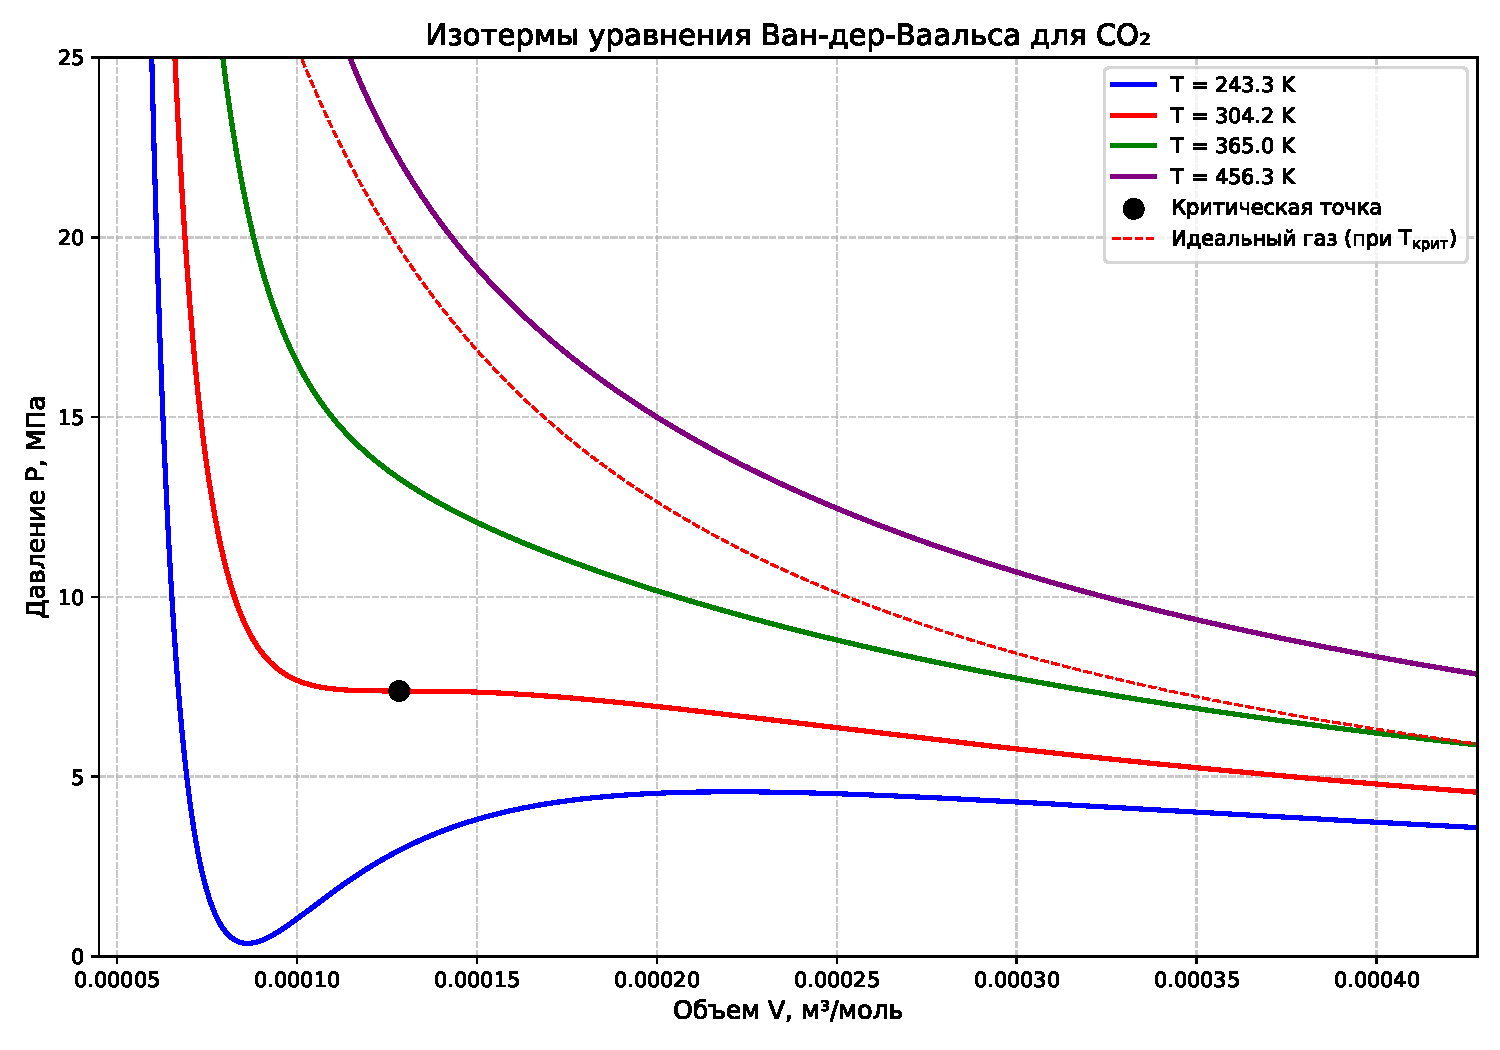
\includegraphics[scale=0.7]{Ван.pdf}}
    \end{figure}
    \begin{figure}[ht]
        \center{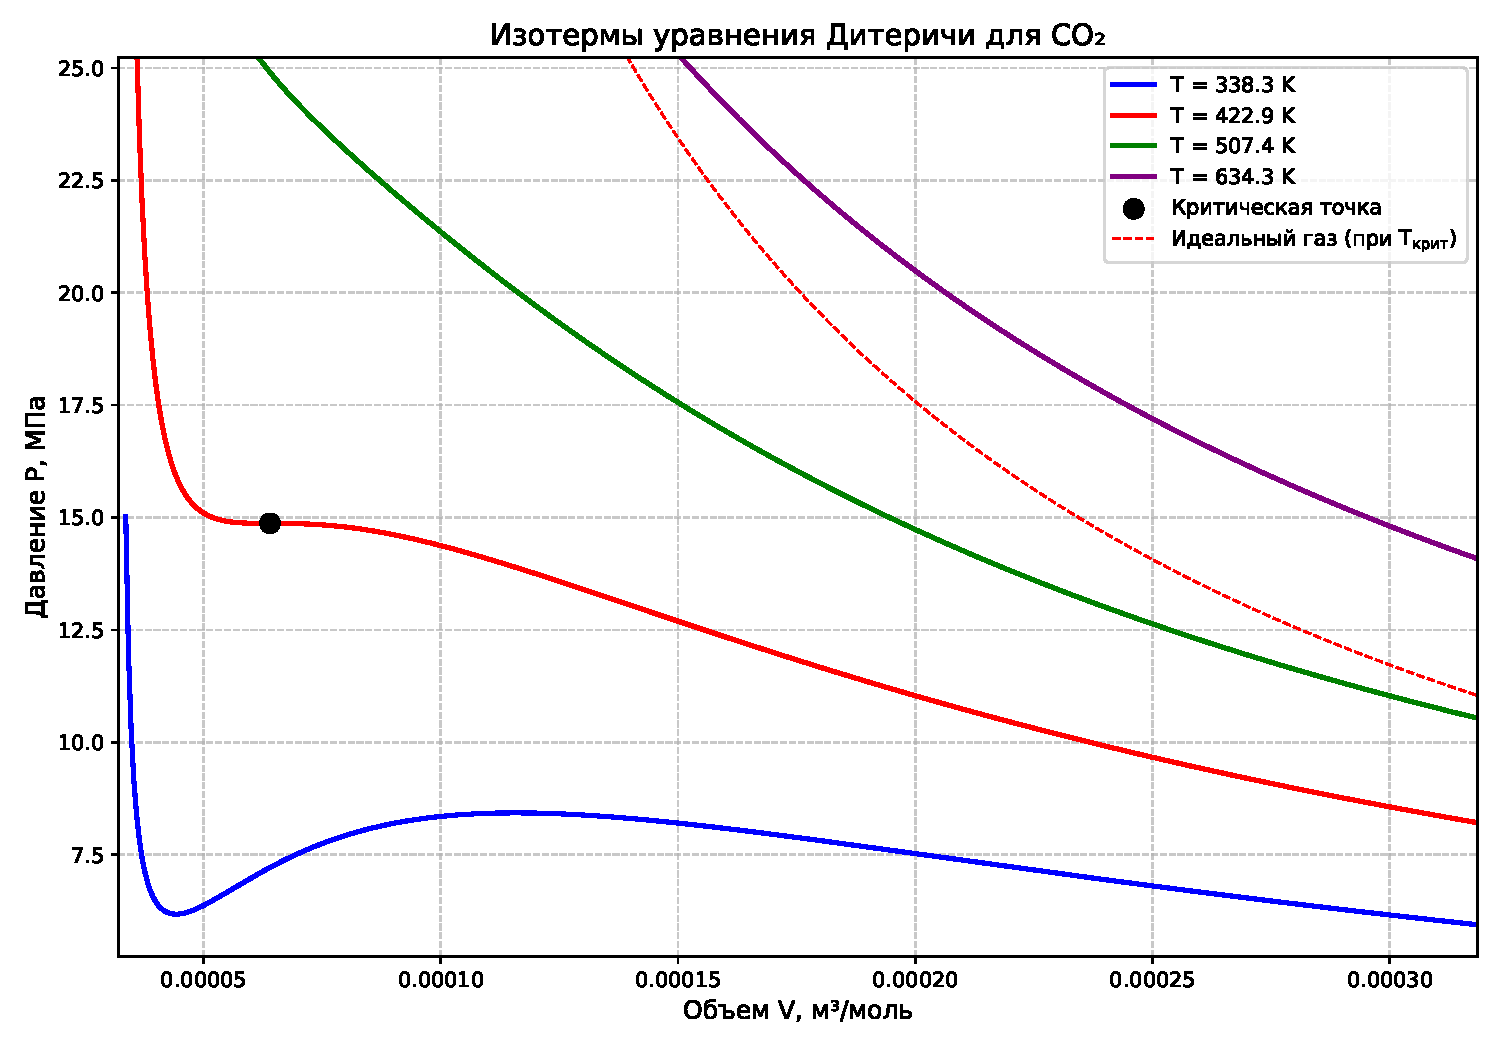
\includegraphics[scale=0.7]{Дит.pdf}}
    \end{figure}
    \begin{figure}[ht]
        \center{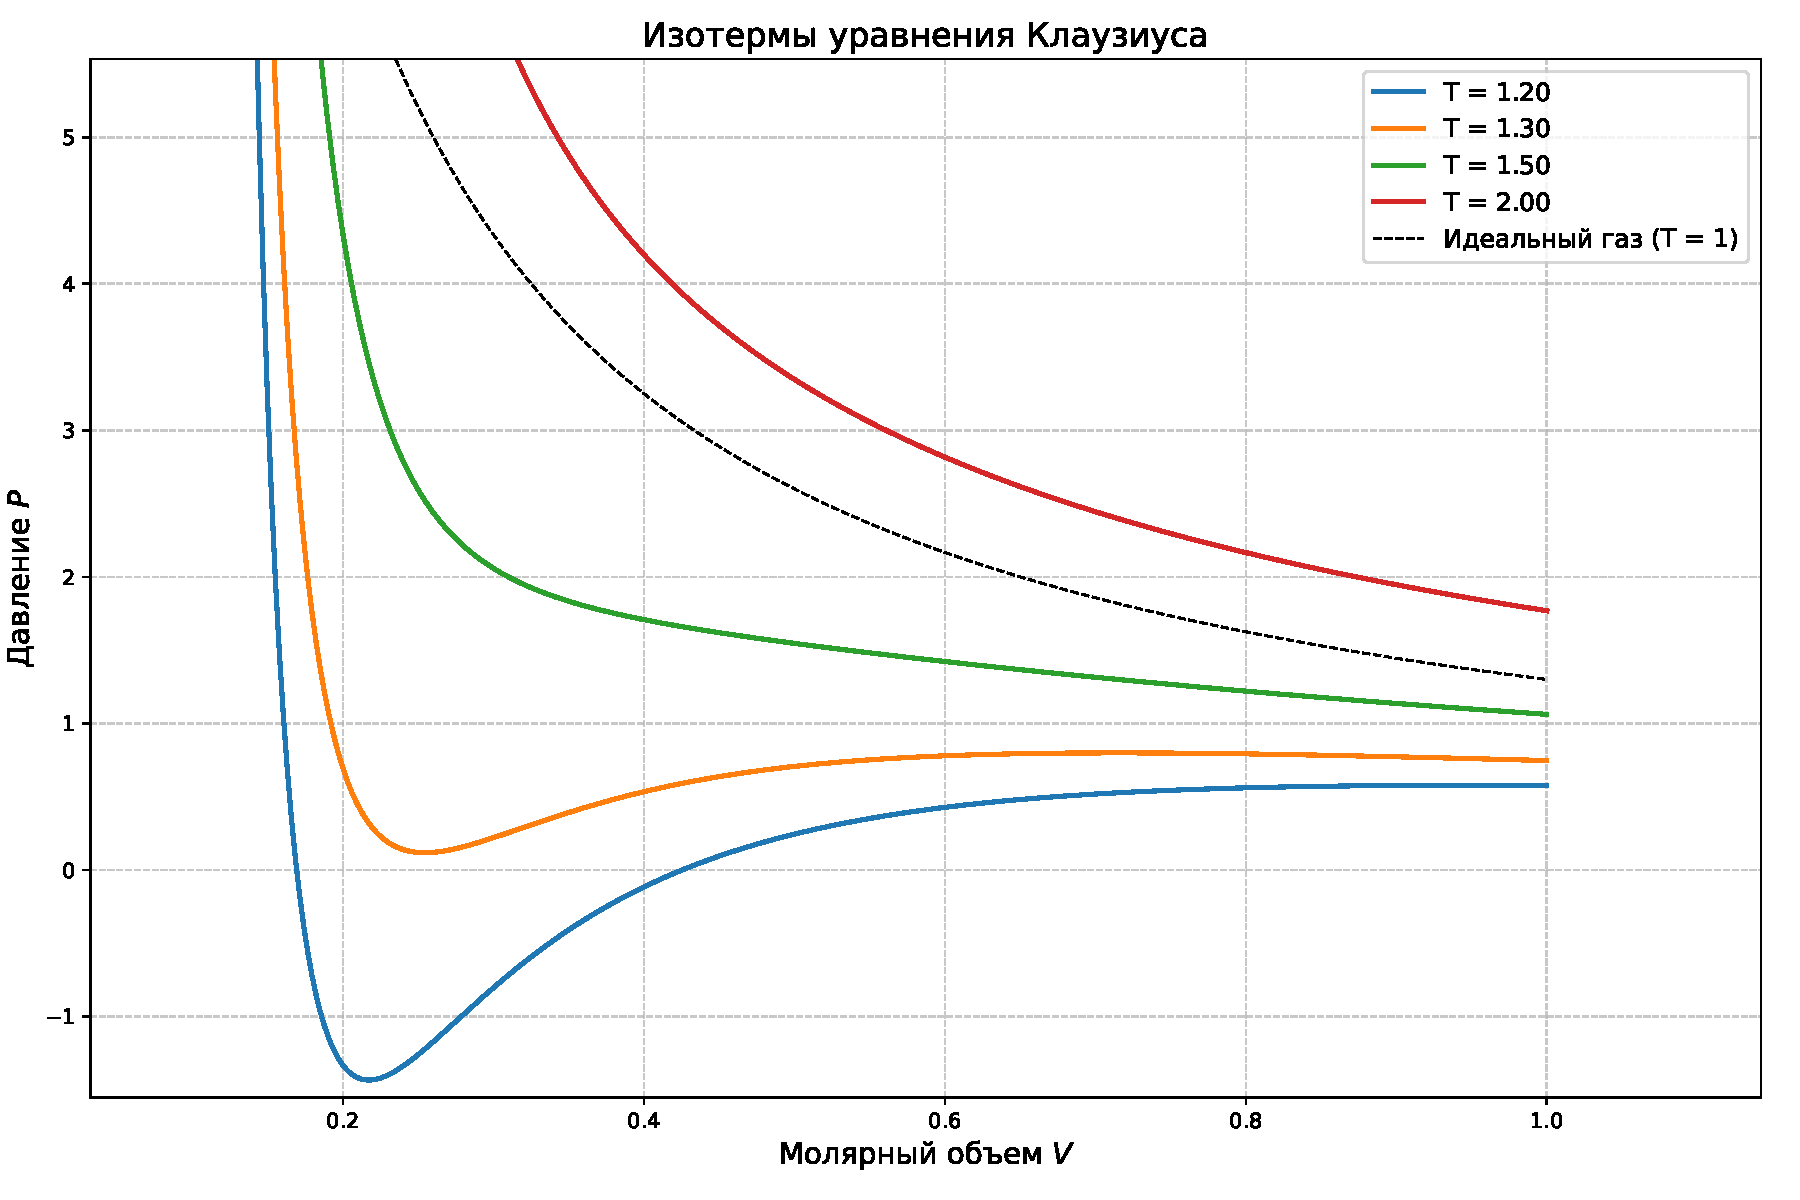
\includegraphics[scale=0.55]{Клауз.pdf}}
    \end{figure}
        \begin{figure}[ht]
        \center{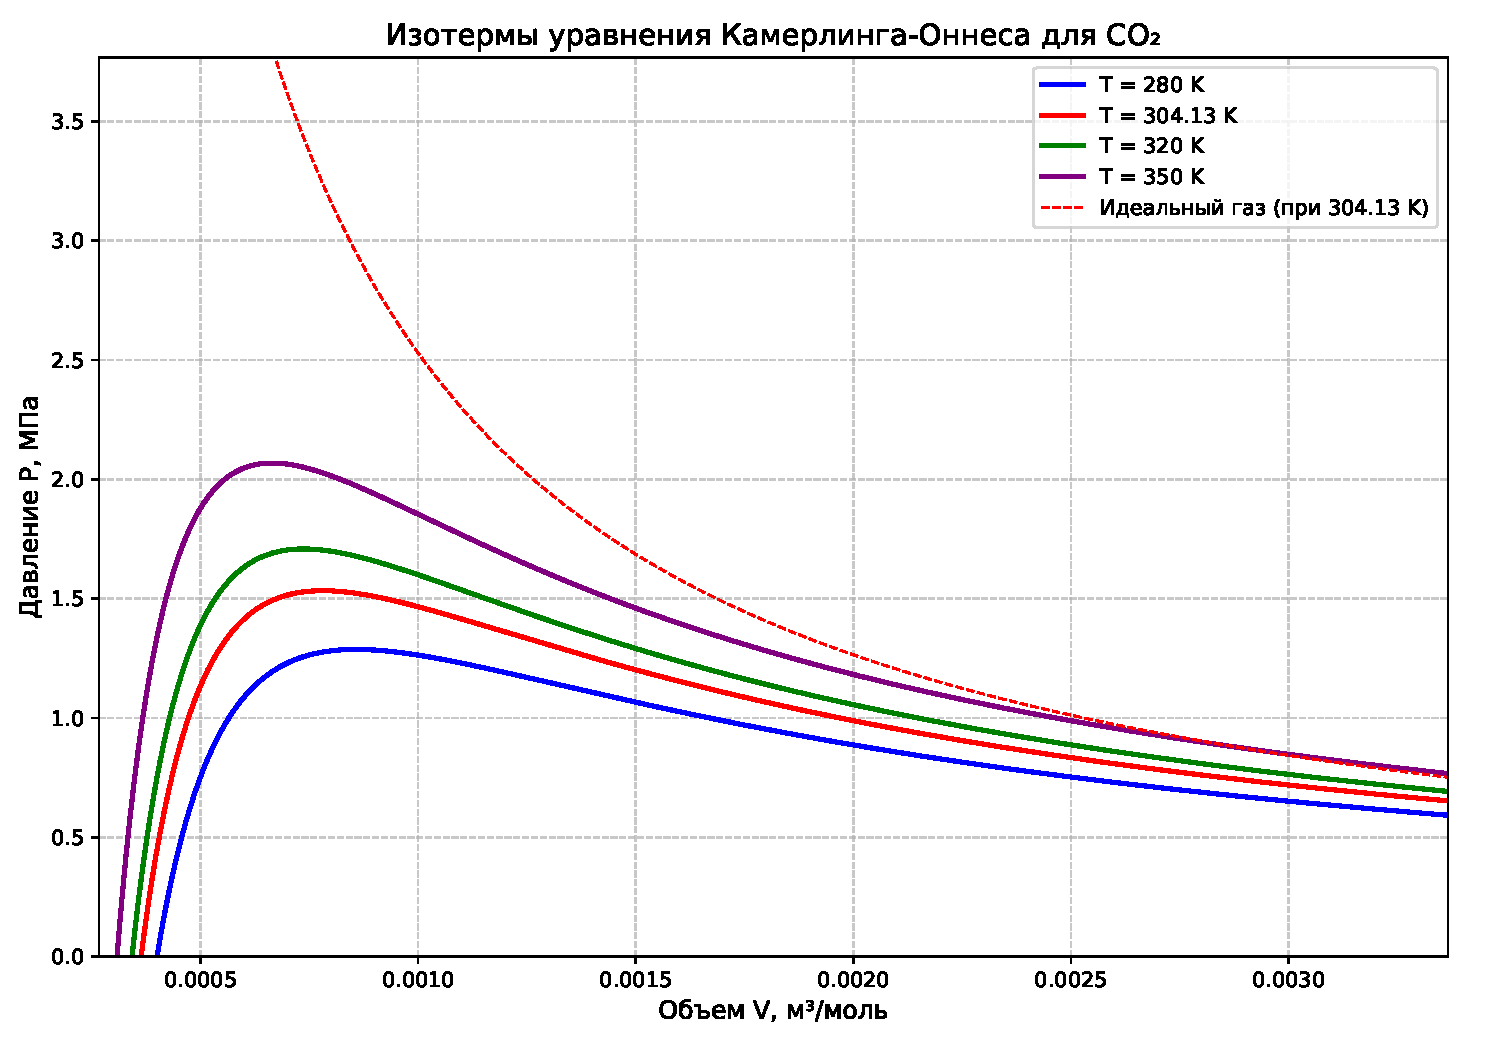
\includegraphics[scale=0.7]{Кам.pdf}}
    \end{figure}


\end{document}